\section{Softwaredesign} % (fold)
\label{sec:softwaredesign}

Um den Code leicht erweitern zu können und Fehlern vorzubeugen, ist es wichtig, den Aufbau der Software gut zu strukturieren. Dabei gibt es einige typische Probleme, für die bereits etablierte Lösungen existieren. Diese Design Pattern helfen nicht nur dabei, den Code wartbar zu halten, sondern helfen auch in der Kommunikation mit anderen Entwicklern bei strukturellen Problemen. In diesem Kapitel soll ein Highlevel-Überblick über die Softwarestruktur und verwendete Design Muster gegeben werden.

\subsection{Model View Controller} % (fold)
\label{sub:model_view_controller}
Eines der wohl am weitesten verbreitete Entwurfsmuster ist das Model View Controller Pattern, das auch in dieser Arbeit umgesetzt wurde. Es trennt die verschiedenen Aufgaben einer Software in drei Bereiche auf: Daten und Spiellogik bilden das Modell, das in sich funktioniert und nach außen Schnittstellen bietet, die dann interne Spielprozesse auslösen. Getrennt davon ist die View, deren Aufgabe einzig darin besteht, die Daten aus dem Modell (evtl. gefiltert) dem Spieler anzuzeigen. Diese View ist mit JavaFX geschrieben, wobei die Trennung vom restlichen Code teilweise durch die Verwendung von \emph{FXML} besonders deutlich wird. Die View muss dabei Änderungen aus dem Modell mitbekommen und daraufhin entsprechend anzeigen. Die View stellt zudem Schnittstellen zur Verfügung, um auf bestimmte Useraktivitäten zu reagieren. Diese Schnittstellen verwendet der Controller. Er setzt also Listener auf Komponenten der View für verschiedene User Interaktionen wie Mausklicks, Hovering oder Tastatureingaben. Die Listener sind größtenteils als anonyme Klassen implementiert und rufen bei einer Aktion die entsprechenden Schnittstellen des Modells auf.  
% subsection model_view_controller (end)

\subsection{Observer Pattern} % (fold)
\label{sub:observer}
Im Zusammenspiel mit MVC ist das Observer Pattern eines der wichtigsten. Es ermöglicht eine lose Kopplung zwischen View und Modell, indem sich die View beim Modell als Observer registriert und das Modell bei Änderungen alle Observer benachrichtigt. Dadurch ist gewährleistet, dass das Modell nicht explizit die View kennen muss und so kann die View leichter ausgetauscht werden oder weitere Views (z.B. auch Sounds) angebunden werden, ohne in das Modell einzugreifen. In JavaFX funktioniert die Umsetzung ein wenig anders, nämlich mittels \enquote{Bindings}: Das Modell bietet Properties an, auf denen Listener registriert werden können, die aber auch direkt an Viewausgaben gebunden werden können. Beispielsweise stellt die Geldanzeige im Spiel einen formatierten String der \class{IntegerProperty money} des \class{PlayerModel} dar. Da immer das aktuelle Geld angezeigt werden soll, kann hierfür ein Binding verwendet werden, statt den Umweg über einen Listener zu nehmen.
% subsection observer (end)

\subsection{Game Loop} % (fold)
\label{sub:gameloop}
Eine Game Loop löst das Problem, die Spielzeit mit der Realzeit zu synchronisieren, statt ihren Ablauf von User-Interaktionen (wie bei klassischen EVA), abhängig zu machen oder von der Prozessorgeschwindigkeit abhängig zu sein \cite{gameloopPattern}. Die Implementierung richtet sich nach \cite{gameloopImpl, gameloopImplFX} und verwendet drei Elemente:
\begin{itemize}
	\item \textbf{Synchronisation mit der Realzeit}: Messe wie viel Realzeit seit der letzten Spielzeit Simulation vergangen ist und simuliere ungefähr diese Zeitspanne (Einschränkungen siehe die nächsten zwei Punkte).

	\item \textbf{Feste Zeitschritte}: Eine Frame Rate über 60 Bilder pro Sekunde ist nicht notwendig, daher wird versucht diese Zielrate ungefähr zu erreichen. Kürzere Zeitschritte werden also zusammengefasst, bis \(1/60\) Sekunde zusammenkommen, größere Zeitschritte werden in mehrere 1/60 Sekunden Schritte zerteilt und einzeln simuliert. Dadurch bleibt das Spiel deterministisch -- im Gegensatz zur Verwendung von variablen Zeitschritten.

	\item \textbf{Begrenzte Zeitschritte}: Ist der Prozessor zu langsam, um eine Iteration in \(1/60\,s\) auszuführen, ist bei der nächsten Iteration mehr Zeit vergangen, wodurch er mehr Zeitschritte machen muss, die wieder länger dauern, etc. Um diese Spirale zu verhindern, wird die vergangene Zeit auf eine bestimmte Länge beschränkt. Die Nachteil daran ist, dass das Spiel auf zu langsamen Prozessoren langsamer läuft.
\end{itemize}

Interpolation der Zeitschritte wurde nicht eingebaut, da diese Komplexität sich in alle Komponenten fortsetzt, die von der Game Loop synchronisiert werden sollen.

Wegen JavaFX wurde die \class{GameLoop} als Spezialisierung des \class{AnimationTimer} erstellt, der automatisch durch den JavaFX-Thread aufgerufen wird. Durch das Binding konnten die Zeitupdates der View aus der Game Loop entfernt werden, da sie bei Änderungen des Modells bereits ihre internen Werte ändern und vom JavaFX-Thread aktualisiert werden.
% subsection gameloop (end)

\subsection{Strategy Pattern} % (fold)
\label{sub:strategy_pattern}
Das Strategy Pattern wird verwendet, um den Ablauf eines Algorithmus zur Laufzeit ändern zu können. Man erstellt Objekte, die die Implementierung des Algorithmus beinhalten und verwendet dann Komposition der Objekte. Dadurch können auch viele unterschiedliche Algorithmen für die selbe Klasse implementiert werden, ohne Unterklassen zu verwenden. Dies entspricht auch dem Prinzip der Objekt Orientierung \enquote{composition over inheritance}, durch das eine lose Kopplung erreicht werden kann. Verwendet wurde dieses Pattern bei der Wegfindung der Creeps. Die Klasse \class{RandomMovement} implementiert eine völlig zufällige Bewegung und Berücksichtigt nur Wände. Diese wird von den einfachsten Kreaturenarten verwendet, die nur am Anfang auftauchen. Dagegen sucht \class{NoSightMovement} mit einer abgewandelten Dijkstra-Suche das nächste unbekannte Feld (bezieht also bereits besuchte Felder ein) und bewegt sich zu diesem hin. Dabei werden jedoch nur Felder auf besucht gesetzt, die tatsächlich abgelaufen wurden. Eine weitere mögliche Klasse, die nicht mehr implementiert wurde, ist \class{SightMovement}, die alle Felder auf besucht setzt, die von der aktuellen Position aus gesehen werden können und erst dann nach einem unbekannten Ziel sucht. Ebenso wäre eine Klasse \class{PerfectMovement} denkbar, die dem kürzesten Weg zum Ziel durch das Labyrinth verfolgt, wie es normalerweise in Tower Defense Spielen üblich ist.

\begin{figure}[htb]
	\centering
	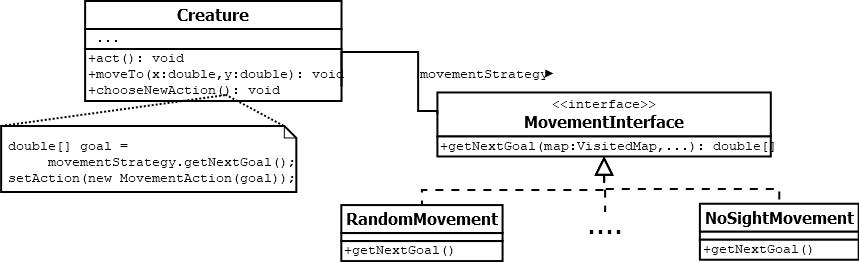
\includegraphics[width=\linewidth]{images/strategy-pattern.png}
	\caption{Strategy Pattern bei der Wegfindung}
\end{figure}

Dass diese Algorithmen zur Laufzeit ersetzt werden können, bietet die Möglichkeit für interessante Kreaturen-Interaktionen und Tower-Arten: Mit dem \class{AmnesiaTower} wurde ein Turm implementiert, der die Creeps durch seine Schüsse verwirrt. Dabei ersetzt er für eine kurze Zeit den eigentlichen Wegfindungsalgorithmus der Kreatur durch \class{RandomMovement}. Genauso könnte man Creeparten implementieren, die anderen beim Kommunizieren bessere Strategien beibringen, also z.B. \class{RandomMovement} der einfachsten Kreaturen durch \class{SightMovement} ersetzen. Ebenfalls angedacht sind Kommandeure, die -- statt selbst durch das Labyrinth zu rennen -- auf Türme klettern und von dort mit Überblick über das gesamte Labyrinth die anderen Creeps durchlotsen können, also die Bewegung durch \class{PerfectMovement} ersetzen. 

Auch Algorithmusimplementierungen, die gar nicht darauf abzielen das Labyrinth zu durchqueren, wären möglich. Beispielsweise könnten intelligentere Kreaturen an geschützten Stellen warten oder priorisiert zu anderen Kreaturen laufen, um diesen Informationen weiterzugeben. Das Projekt bietet hier wie man sieht noch einige Erweiterungen, die bisher noch nicht implementiert werden konnten. Die Grundfunktionalität, um solche Features umzusetzen, sind allerdings mit dem Strategy Pattern gelegt und am Beispiel des Amnesie-Turms auch verwendet.
% subsection strategy_pattern (end)


\subsection{Static Factory Method} % (fold)
\label{sub:static_factory_method}
Gemeint ist hier nicht das Factory Method Pattern, sondern eine statische Methode zur Erzeugung eines Objektes einer Klasse. Im Gegensatz zum Konstruktor hat die Static Factory Method die Möglichkeit auch Objekte von Unterklassen zu erzeugen oder ein bereits erzeugtes Objekt zurückzugeben \cite[5 ff.]{Bloch2008}. In diesem Sinne verwendet z.B. auch das Singleton Pattern eine Static Factory Methode. Dieses Vorgehen wurde sowohl für Türme verwendet, bei denen der Aufruf konkrete Objekte der Unterklassen erzeugt, sowie für die Kreaturen. Bei letzteren ist die Erzeugung etwas umfangreicher und mit verschiedenen Parametern möglich und wurde zur Übersichtlichkeit daher in eine eigene Klasse \class{CreatureFactory} ausgelagert. Diese Factory kann dann z. B. anhand des Types und des Zeitfortschritts die Leben und den Wert der Creeps, sowie deren Bewegungsstrategie bestimmen und entsprechend den Konstruktor der \class{Creature} aufrufen. Dadurch wird die Erzeugung der Figuren besser gekapselt.

% subsection static_factory_method (end)
% section softwaredesign (end)